\chapter{Versuchsaufbau}
\section{Einleitung}

\begin{figure}[H]
    \centering
    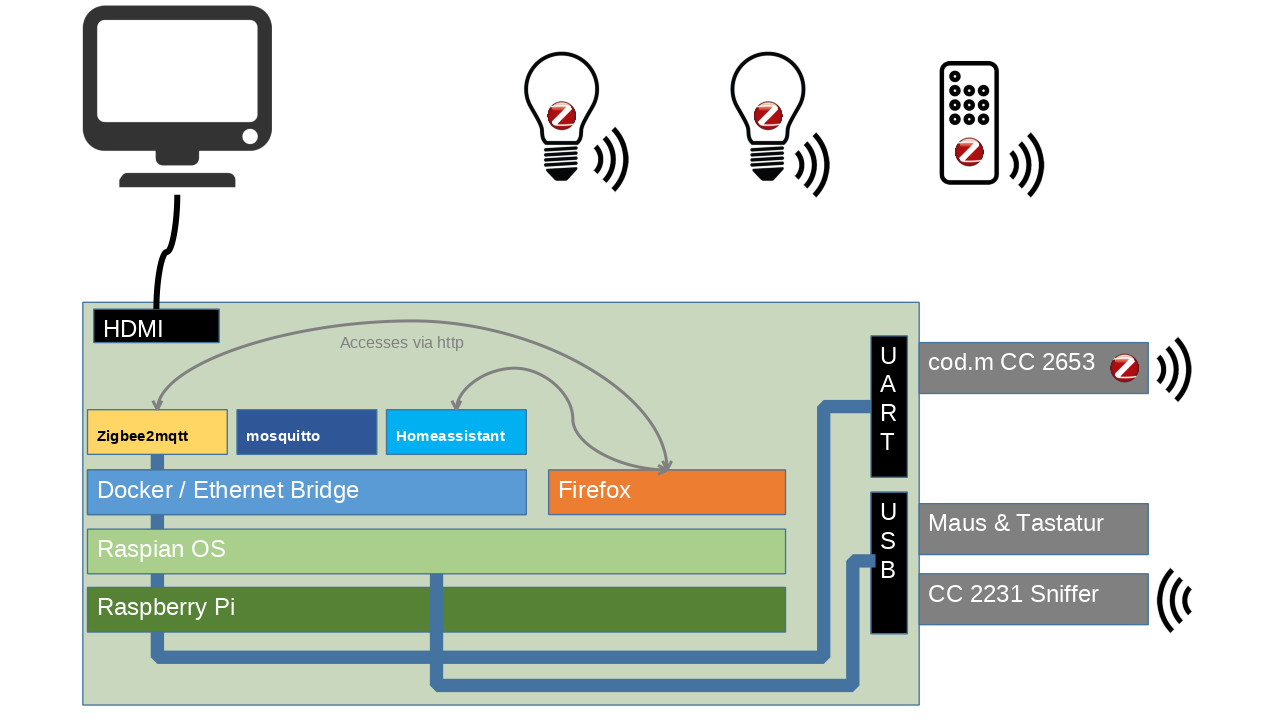
\includegraphics[width=1\textwidth]{media/Versuchsaufbau/image1.png}
    \caption{Versuchsaufbau}
  \end{figure}

In dieser Abbildung wird der schematische Versuchsaufbau gezeigt. Die drei Anwendungen werden als Docker Container ausgeführt. Sie kommunizieren
untereinander über ein eigenes Docker Netzwerk. Dies ist eine von Docker verwaltete Linux Bridge. Nur der NGINX Reverse Proxy hat zwei Ports, die
auf die Host Schnittstelle gemappt werden. Die Webfrontends sind damit über den lokal installierten Browser über das Loopback-Interface erreichbar. Damit ist der Raspberry Applikationsserver
und Versuchs-PC zugleich.

Es werden entsprechende Namen in der lokalen \grqq hosts\grqq{} Konfigurationsdatei hinterlegt, um lokal Domainnamen auflösen zu können.

Der cod.m Zigbeecontroller wird direkt an den Docker Container durchgereicht. Der Sniffer Stick ist regulär am Host angeschlossen. 

\section{Containerverwaltung}



\subsection{Nginx Proxy}
\begin{lstlisting}
    proxy:
      container_name: nginx
      image: jwilder/nginx-proxy:alpine
      networks:
        - backbone
      ports:
        - 80:80
        - 443:443
      volumes:
        - ./NGINX/proxy/conf.d:/etc/nginx/conf.d:rw
        - ./NGINX/proxy/vhost.d:/etc/nginx/vhost.d:rw
        - ./NGINX/proxy/html:/usr/share/nginx/html:rw
        - ./NGINX/proxy/certs:/etc/nginx/certs:ro
        - /etc/localtime:/etc/localtime:ro
        - /var/run/docker.sock:/tmp/docker.sock:ro
      restart: unless-stopped
\end{lstlisting}

Der Proxy basiert auf einem Image des Proxys NGINX \cite{nginxpm}. Vorteil dieses erweiterten NGINX ist es,
dass dieser automatisiert seine Konfigurationen verwaltet. Dafür wird bei einem Service eine entsprechende Umgebungsvariablen gesetzt. Über den 
\grqq docker.sock\grqq{} erfährt der Proxy ob Container gestartet werden sowie deren Umgebungsvariablen. Wird ein Container mit der Umgebungsvariable 
\grqq VIRTUAL\_HOST=z2m.local \grqq{} gestartet, wird automatisch eine Weiterleitung für alle Anfragen mit dem Header \grqq z2m.local\grqq{} eingerichtet auf den entsprechenden Container.
Alle Servicecontainer sind in einer eigenen L2-Domäne und von außen nicht direkt erreichbar. Der Proxy Container ist der einzige, dem externe Ports zugewiesen werden.
Dafür werden von Docker Regeln in die \grqq iptables \grqq{} Tabellen geschrieben.

\begin{figure}[H]
  \centering
  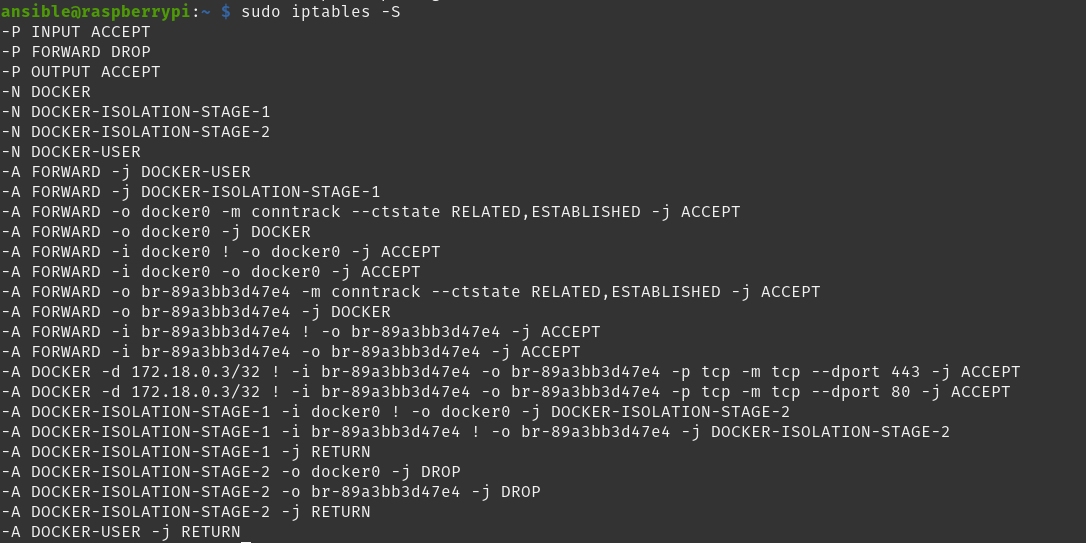
\includegraphics[width=1\textwidth]{media/rasp-iptables.png}
  \caption{Raspberry iptables}
\end{figure}

Die Regeln in der Tabelle \grqq DOCKER \grqq{} werden durch Docker geschrieben. Eigene Regeln können in der Tabelle 
\grqq DOCKER-USER \grqq{} definiert werden.

\begin{figure}[H]
  \centering
  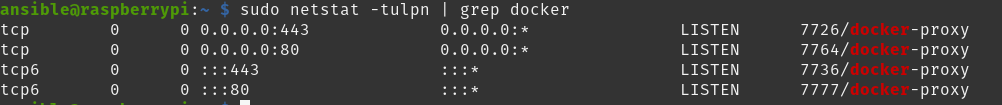
\includegraphics[width=1\textwidth]{media/rasp-netstat.png}
  \caption{Raspberry netstat}
\end{figure}

In dieser Ausgabe ist erkennbar, dass Docker auf die Ports 80 und 443 lauscht.

\subsection{zigbee2mqtt}
\begin{lstlisting}
  zigbee2mqtt:
    container_name: zigbee2mqtt
    image: koenkk/zigbee2mqtt
    networks:
      - backbone
    volumes:
      - ./Z2M/data:/app/data
    devices:
       - /dev/ttyAMA0:/dev/ttyAMA0
    restart: always
    environment:
      - VIRTUAL_HOST=z2m.local
      - VIRTUAL_PORT=8080
    group_add:
      - dialout
\end{lstlisting}

Dem Container wird ebenfalls das Netzwerk \grqq backbone\grqq{} zugewiesen. Ein Verzeichnis mit Konfigurationen und persistenten Datensätzen wird auf den Host gemountetn. Wenn der gemountete Pfad außerhalb des Containers nicht existiert, wird der 
bestehende Ordner aus dem Container kopiert. Exisitert der Pfad, wird der Ordner vom Host in den Container gemountet. 
Bei Linux können Geräte über das selbe Verfahren wie Verzeichnisse adressiert werden. \grqq - /dev/ttyUSB0:/dev/ttyACM0\grqq{} reicht den ZigBee Adapter an 
den Docker Container weiter.
In den Umgebungsvariablen wird dem Proxy noch mitgeteilt, unter Welcher URL er erreichbar sein soll und auf welchem Port der Webserver läuft. Die Gruppe 
\grqq dialout\grqq{} ist notwendig, damit der Container Zugriffsrechte auf die serielle Schnittstelle des Hosts erhällt.

Folgend die zentrale Konfigurationsdatei von \grqq zigbee2mqtt\grqq{}.
\begin{lstlisting}
homeassistant: true
permit_join: false
mqtt:
  base_topic: zigbee2mqtt
  server: mqtt://mosquitto:1883
serial:
  port: /dev/ttyACM0
frontend:
  port: 8080
  host: 0.0.0.0
  url: https://z2m.local
advanced:
  homeassistant_legacy_entity_attributes: false
  legacy_api: false
  legacy_availability_payload: false
device_options:
  legacy: false
\end{lstlisting}

Es wird der \grqq Homeassistant\grqq{} Modus aktiviert, Damit werden die Nachrichten an den MQTT Broker für Homeassistant verständlich gestaltet.
Das Beitreten neuer Geräte ist standardmäßig deaktiviert und muss explizit erlaubt werden. Desweiteren wird ein MQTT Server angegeben, sowie ein \grqq base-topic\grqq{}
definiert. Docker löst Containernamen in Dockernetzwerken zu IP-Adressen auf, sodass hier als Server der entsprechende Containernamen angegeben werden
kann. Im weiteren wird der Pfad angegeben, auf den der cod.m Adapter gemountet wurde, sowie entsprechende Einstellung für den Webserver gesetzt.

\subsection{mosquitto}

\begin{lstlisting}
  mosquitto:
  container_name: mosquitto
  image: eclipse-mosquitto:latest
  networks:
    - backbone
  restart: always
  deploy:
    resources:
      limits:
        memory: 125M
  volumes:
    - ./mosquitto/config:/mosquitto/config
    - ./mosquitto/data:/mosquitto/data
    - ./mosquitto/log:/mosquitto/log
\end{lstlisting}

Als MQTT Broker wird \grqq mosquitto\grqq{} eingesetzt. Die Konfigurationen 
wurden auch hier entsprechend auf den Host gemountet. Als Konfigurationsdatei wird das Standardtemplate verwendet, welches nur an zwei 
entsprechenden Stellen modifiziert ist.

\begin{lstlisting}
... 
allow_anonymous true
... 

... 
listener 1883
... 
\end{lstlisting}

Es wird der Zugriff von nicht authentifizierten Geräten erlaubt. Dies stellt kein Risiko dar, da der Container nur innerhalb des \grqq backbone\grqq{} 
Netwerkes sowie vom Host selber erreichbar ist. Zusätzlich wird der Port definiert, auf dem der MQTT Service läuft. 1883 ist der standard Port für MQTT.

\section{Namensauflösung}

Für eine lokale Namensauflösung werden die Hosts in die \grqq \textbackslash etc\textbackslash hosts\grqq{} eingetragen. Dies wird automatisch in der Ansible
Rolle \grqq DeployLab\grqq{} gemacht.

\begin{lstlisting}
- name: Add Hosts Entrys
  become: True
  lineinfile:
    path: /etc/hosts
    line: 127.0.0.1 z2m.local
\end{lstlisting}

\section{Anwendungen}

Für den Versuch wird weiterhin ein Webbrowser sowie Wireshark benötigt. Die beiden Anwendungen werden per Ansible installiert:
\begin{lstlisting}
  - name: Install required Packages
  become: true
  apt:
    pkg:
      - wireshark
      - firefox
    state: latest
    update_cache: true
\end{lstlisting}

